%++++++++++++++++++++++++++++++++++++++++
% Don't modify this section unless you know what you're doing!
\documentclass[letterpaper,12pt]{article}
\setlength{\parindent}{4ex}
\setlength{\parskip}{1ex}

\usepackage{graphicx}
\usepackage{indentfirst}
\usepackage{tabularx} % extra features for tabular environment
\usepackage{subfigure} 

\usepackage{caption} % Spacing between caption (title) and actual table
\captionsetup[table]{skip=10pt}

\usepackage{amsmath}  % improve math presentation
\usepackage{graphicx} % takes care of graphic including machinery
\usepackage{pgfplots}
\usepackage[margin=1in,letterpaper]{geometry} % decreases margins
\usepackage{cite} % takes care of citations
\usepackage[final]{hyperref} % adds hyper links inside the generated pdf file
\hypersetup {
	colorlinks=true,       % false: boxed links; true: colored links
	linkcolor=blue,        % color of internal links
	citecolor=blue,        % color of links to bibliography
	filecolor=magenta,     % color of file links
	urlcolor=blue         
      }
      \setcounter{tocdepth}{3}

\usepackage{pgfplots}      


% ++++++++++++++++++++++++++++++++++++++++

\begin{document}

\title{CS 7641 Machine Learning \\
		\ Assignment 1 }
\author{David Yun}
\date{September 23, 2018}
\maketitle

\begin{abstract}
  The implementation (in Python2.6 or Python3, depending on the algorithm), and basic fundamentals behind the following Machine Learning Algorithms will be discussed in detail:  
  \begin{enumerate}
  \item Decision trees with some form of pruning
  \item Boosting
  \item Support Vector Machines (SVM)
  \item k-Nearest Neighbors (kNN)
  \item Neural Networks
  \end{enumerate}

  The full code files are available on github\footnote{David Yun's Github: \url{https://github.com/tree-fiddy/Assignment_1}}
  Please refer to the README.txt file for concise instructions on how to run the python files associated with each of the aforementioned algorithms.  Further details behind the datasets, including where to download them, are provided in the README.  

\end{abstract}

\tableofcontents

\section{Datasets}
The two datasets used are both sourced from the UCI Machine Learning Repository.  The first one, the \href{http://archive.ics.uci.edu/ml/datasets/credit+approval}{Credit Approval Data Set} is a smaller dataset with 690 instances, and 15 attributes.  As a full time employee at American Express, credit approval is highly relevant to my job.  As such, I wanted to take this opportunity to see how Machine Learning can be directly applied to credit approval data.  The second dataset, the \href{https://archive.ics.uci.edu/ml/datasets/MoCap+Hand+Postures#}{MoCap Hand Postures Data Set} is a much larger dataset with 78,095 instances, and 38 features.  This dataset classifies 5 different hand gestures using 11 markers attached to each finger of a glove in a motion capture environment.  The application of Machine Learning here is interesting because it provides a rudimentary step in the direction towards Virtual Reality- a burgeoning field directly applying Machine Learning to read \& track objects.

I thought it would behoove me to use two very different datasets, both in scope, and size, to truly gain an understanding of the usefulness of Machine Learning.  Not all models are built the same, and not all datasets benefit from a given model.  Thus, getting the opportunity to apply the same, or similar, models on two fundamentally different datasets would help uncover where certain models prove useful, and where the same models might prove inadequate.  

\section{Decision Trees (via Random Forest) \& Boosting}

The accuracy of our decision tree relies on our tolerance for pre-pruning.  In essence, one must specify \emph{when} to stop growing the tree.  On one extreme, we can set a condition to stop growing the tree once we reach a \emph{pure\footnote{A leaf is said to be ``pure'' if the leaf contains homogenous labels.  By extension, this equates to a situation where Entropy equals 0.}} leaf.  However, this will likely make the tree longer than need be.  A more depth-restrictive approach is to set an arbitrary threshold for Entropy in our Decision Tree, where we will halt further node and leaf generation if the current node produces leaves with Entropy values less than our specified threshold.  To ensure the efficacy of our pre-pruning process, we also incorporate a limit to the depth of our tree to 5.  This will handle extreme cases where our dataset is so large, that splitting across many features is possible. This also has the added benefit of dramatic performance improvement, without sacrificing accuracy, when compared to not setting a depth and letting the tree grow indefinitely.

As you can see, the model's accuracy reached an asymptote of around 50\% accuracy for the credit card data, which indicates that setting a higher threshold for Entropy renders this model's efficacy no better than a coin flip. Thus, setting a pre-pruning specification is quite important here. 

Our Boosting code uses the AdaBoost Classifier in sklearn, and uses Decision Trees as weak learners.  We try to find the best model by iterating on different number of estimators (1,2,5,10,20,30,45,60,80,100) and alphas ($-10^{-3}$ to $10^{-3}$). We also iterate on training sample size to see if our model overfits the data, and to find a sufficient training sample size.  In our case, our training accuracy did not converge with the validation set for either data sets.

\subsection{Learning Curves Analysis}

\textbf{Hand Posture Data}:  The large dataset provided very great results using both algorithms.  The Random Forest immediately achievs near 100\% validation accuracy at low values of entropy, whereas Boosting produces a max accuracy of 84\%.  This boils down to Bagging vs. Boosting, and it is clear that our dataset performs much better by averaging the individuals results (Bagging) than by .  It is also worth noting that tuning was a much more straightforward process via Random Forest Decision Trees, compared to Boosting.  For one, tuning the alpha (regularization loss descent rate) was computationally expensive for little benefit, as shown in Figures \ref{fig: Boosting Learning Curve alpha = 0} and \ref{fig: Boosting Learning Curve alpha = -1}.  As a result, I believe a Random Forest might work better with the Hand Posture data because the geospatial location of fingers associated with each hand posture has great discernability- perfectly leveraging the ID3 algorithm's strength in using Information Gain to identify which features discriminate effectively.  


\textbf{Credit Approval Data}: Decision Trees with Random forests allow us to create a robust model with less variance which results in a reduction in overfitting\footnote{By averaging several decision trees, the result is a less likely chance of overfitting}.  With proper pruning (Entropy thresholds \& Max Depth), one can further reduce the variance of the model and further decrease the chance of overfitting.


\begin{table}[htb]
  \caption{Credit Approval: Pre-Pruning Spec Performance (forest size = 50)}
  \label{table:PrePruningTable}
  \centering
  \begin{tabular}{|c|c|c|}
  
    \hline
    \hline
    \multicolumn{1}{c}{Entropy Threshold}
    &  \multicolumn{1}{c}{Model Accuracy} \\
    \cline{1-2}
    0.0 & 0.86 \\
    \cline{1-2}
    0.1 & 0.86 \\
    \cline{1-2}
    0.2 & 0.60 \\
    \cline{1-2}
    0.3 & 0.57 \\
    \cline{1-2}
    0.4 & 0.55 \\
    \cline{1-2}
    0.5 & 0.55 \\
    \cline{1-2}
    0.6 & 0.54 \\
    \cline{1-2}
    0.7 & 0.54 \\
    
    
    \cline{1-2}
  \end{tabular}
\end{table}

\begin{table}[htb]
  \caption{Hand-Posture: Pre-Pruning Spec Performance (forest size = 50)}
  \label{table:Hand_PrePruningTable}
  \centering
  \begin{tabular}{|c|c|c|}
  
    \hline
    \hline
    \multicolumn{1}{c}{Entropy Threshold}
    &  \multicolumn{1}{c}{Model Accuracy} \\
    \cline{1-2}
    0.0 & 0.98 \\
    \cline{1-2}
    0.1 & 0.98 \\
    \cline{1-2}
    0.2 & 0.94 \\
    \cline{1-2}
    0.3 & 0.86 \\
    \cline{1-2}
    0.4 & 0.85 \\
    \cline{1-2}
    0.5 & 0.85 \\
    \cline{1-2}
    0.6 & 0.84 \\
    \cline{1-2}
    0.7 & 0.84 \\
    
    
    \cline{1-2}
  \end{tabular}
\end{table}

\begin{figure}
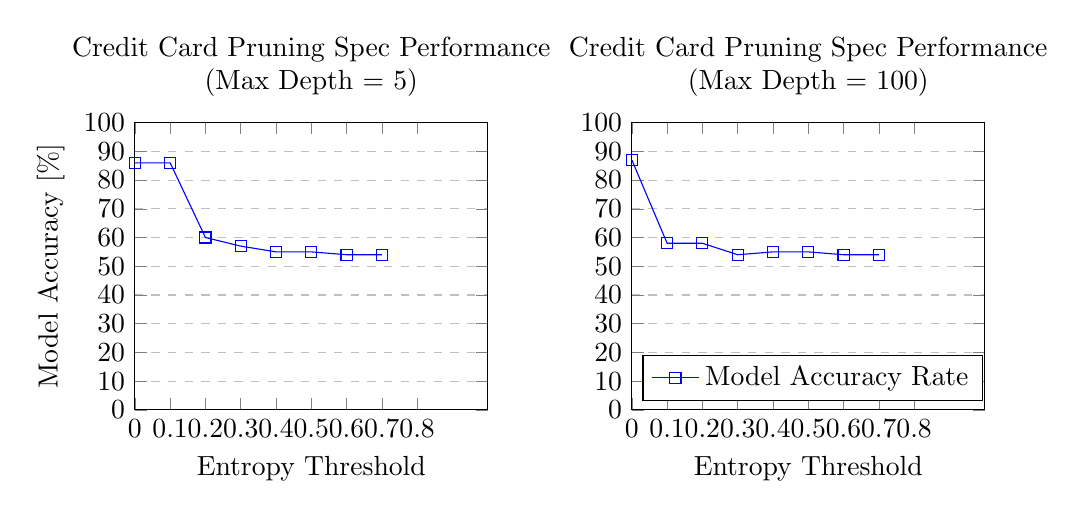
\begin{tikzpicture}[every axis/.append style={width=0.5\linewidth,title style={align=center}}]

  \begin{axis} [
    name = axis1,
    title = {Credit Card Pruning Spec Performance \\ (Max Depth = 5)},
    xlabel = {Entropy Threshold},
    ylabel = {Model Accuracy [\%]},
    xmin = 0, xmax = 1,
    ymin = 0, ymax = 100,
    xtick={0,0.1,0.2,0.3,0.4,0.5,0.6,0.7,0.8},
    ytick={0,10,20,30,40,50,60,70,80,90,100},
    legend pos = south west,
    ymajorgrids=true,
    grid style = dashed
    ]
    \addplot[
    color = blue,
    mark = square,
    ]
    coordinates {
      (0.0,86)(0.1, 86)(0.2, 60)(0.3,57)(0.4,55)(0.5,55)(0.6,54)(0.7,54)
    };
  \end{axis}
  
  \begin{axis} [
    at={(axis1.outer north east)}, anchor=outer north west,
    name=axis2,
    title = {Credit Card Pruning Spec Performance \\ (Max Depth = 100)},
    xlabel = {Entropy Threshold},
    %ylabel = {Model Accuracy [\%]},
    xmin = 0, xmax = 1,
    ymin = 0, ymax = 100,
    xtick={0,0.1,0.2,0.3,0.4,0.5,0.6,0.7,0.8},
    ytick={0,10,20,30,40,50,60,70,80,90,100},
    legend pos = south west,
    ymajorgrids=true,
    grid style = dashed
    ]
    \addplot[
    color = blue,
    mark = square,
    ]
    coordinates {
      (0.0,87)(0.1, 58)(0.2, 58)(0.3,54)(0.4,55)(0.5,55)(0.6,54)(0.7,54)
    };
    \legend{Model Accuracy Rate}
    
 
  \end{axis}
\end{tikzpicture}

\caption{Learning Curves} \label{fig:LearningCurves}
\end{figure}

\begin{figure}
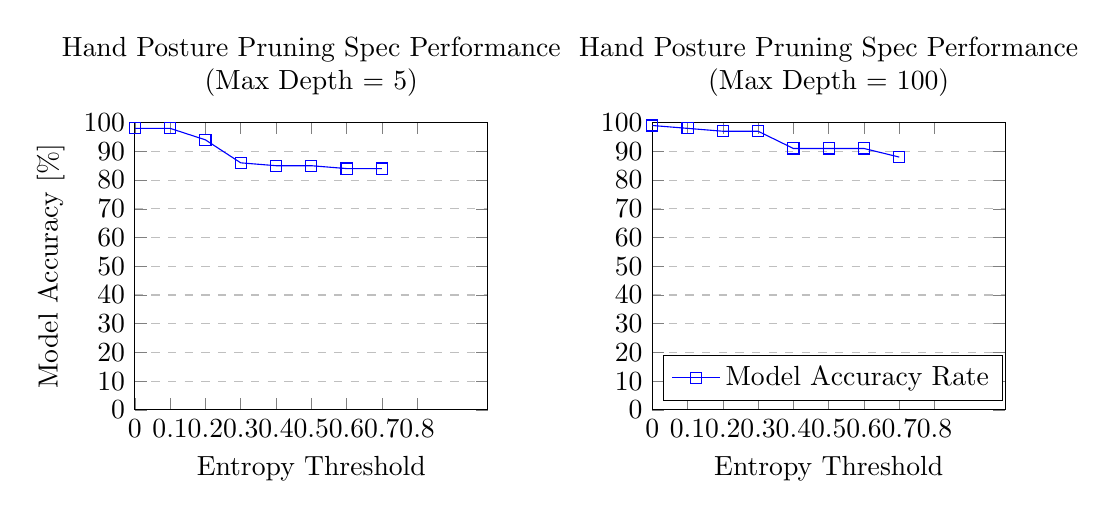
\begin{tikzpicture}[every axis/.append style={width=0.5\linewidth,title style={align=center}}]

  \begin{axis} [
    name = axis1,
    title = {Hand Posture Pruning Spec Performance \\ (Max Depth = 5)},
    xlabel = {Entropy Threshold},
    ylabel = {Model Accuracy [\%]},
    xmin = 0, xmax = 1,
    ymin = 0, ymax = 100,
    xtick={0,0.1,0.2,0.3,0.4,0.5,0.6,0.7,0.8},
    ytick={0,10,20,30,40,50,60,70,80,90,100},
    legend pos = south west,
    ymajorgrids=true,
    grid style = dashed
    ]
    \addplot[
    color = blue,
    mark = square,
    ]
    coordinates {
      (0.0,98)(0.1, 98)(0.2, 94)(0.3,86)(0.4,85)(0.5,85)(0.6,84)(0.7,84)
    };
  \end{axis}
  
  \begin{axis} [
    at={(axis1.outer north east)}, anchor=outer north west,
    name=axis2,
    title = {Hand Posture Pruning Spec Performance \\ (Max Depth = 100)},
    xlabel = {Entropy Threshold},
    %ylabel = {Model Accuracy [\%]},
    xmin = 0, xmax = 1,
    ymin = 0, ymax = 100,
    xtick={0,0.1,0.2,0.3,0.4,0.5,0.6,0.7,0.8},
    ytick={0,10,20,30,40,50,60,70,80,90,100},
    legend pos = south west,
    ymajorgrids=true,
    grid style = dashed
    ]
    \addplot[
    color = blue,
    mark = square,
    ]
    coordinates {
      (0.0,99)(0.1, 98)(0.2, 97)(0.3,97)(0.4,91)(0.5,91)(0.6,91)(0.7,88)
    };
    \legend{Model Accuracy Rate}
    
 
  \end{axis}
\end{tikzpicture}

\caption{Learning Curves} \label{fig:LearningCurves}
\end{figure}

\textbf{Hand Posture}  All the aforementioned patterns hold true for the much larger Hand Posture dataset.  However, the computation was MUCH longer.  While the small credit card approval data took 3 minutes for the highest max depth setting, the Hand Posture data took 3 hours.  You can also see that the accuracy was much higher using this dataset.  Having much more data points probably helped lift accuracy scores, 

\subsection{Model Complexity Analysis}
Besides varying the Entropy Threshold \& Max Depth, we can also vary the \textbf{forest size} hyperparameter in our random forest.  Note here that we vary the hyperparameter, while holding the Entropy Threshold to 0.1 as supported by Figure \ref{fig:MCCurves}.  Note that the \textbf{Credit Card Data} doesn't really improve much with 10x more trees.  However, the same isn't true with the much larger \textbf{Hand Posture Data}, where we see a meaningful improvement in performance as the number of trees is allowed to increase.

\textbf{Hand Posture Data}  To assess the impact of our hyperparamters, I adjust the alpha to -1, learning rate to 0.02, and increase the number of estimators to 20.  Figure \ref{fig: Boosting w/ Hyperparameters 1} shows no discernable difference between the previous two results, which could be due to being ``stuck'' at a local minima and not finding the global minima of the loss function in the gradient descent step.  However, even after setting the learning rate hyper parameter to an exaggerated number (100) yielded similar results, as shown in \ref{fig:Boosting w/ Hyperparameters 2}.


\begin{figure}
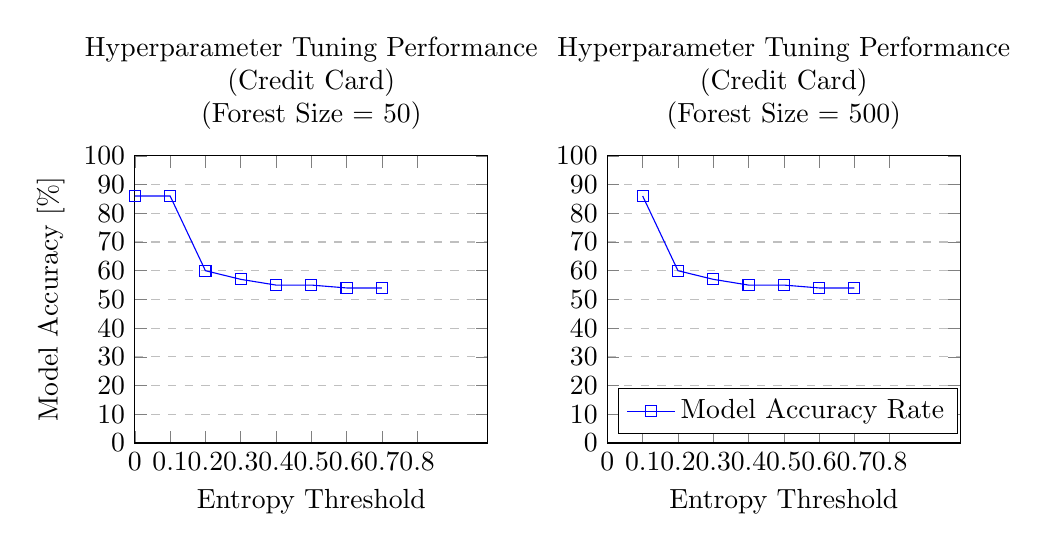
\begin{tikzpicture}[every axis/.append style={width=0.5\linewidth,title style={align=center}}]

  \begin{axis} [
    name = axis1,
    title = {Hyperparameter Tuning Performance \\(Credit Card) \\ (Forest Size = 50)},
    xlabel = {Entropy Threshold},
    ylabel = {Model Accuracy [\%]},
    xmin = 0, xmax = 1,
    ymin = 0, ymax = 100,
    xtick={0,0.1,0.2,0.3,0.4,0.5,0.6,0.7,0.8},
    ytick={0,10,20,30,40,50,60,70,80,90,100},
    legend pos = south west,
    ymajorgrids=true,
    grid style = dashed
    ]
    \addplot[
    color = blue,
    mark = square,
    ]
    coordinates {
      (0.0,86)(0.1, 86)(0.2, 60)(0.3,57)(0.4,55)(0.5,55)(0.6,54)(0.7,54)
    };
  \end{axis}
  
  \begin{axis} [
    at={(axis1.outer north east)}, anchor=outer north west,
    name=axis2,
    title = {Hyperparameter Tuning Performance \\ (Credit Card) \\ (Forest Size = 500)},
    xlabel = {Entropy Threshold},
    %ylabel = {Model Accuracy [\%]},
    xmin = 0, xmax = 1,
    ymin = 0, ymax = 100,
    xtick={0,0.1,0.2,0.3,0.4,0.5,0.6,0.7,0.8},
    ytick={0,10,20,30,40,50,60,70,80,90,100},
    legend pos = south west,
    ymajorgrids=true,
    grid style = dashed
    ]
    \addplot[
    color = blue,
    mark = square,
    ]
    coordinates {
      (0.1,86)(0.1, 86)(0.2, 60)(0.3,57)(0.4,55)(0.5,55)(0.6,54)(0.7,54)
    };
    \legend{Model Accuracy Rate}
  \end{axis}

    
\end{tikzpicture}

\caption{Model Complexity Curves (Credit Card Data)} \label{fig:MCCurves}
\end{figure}

\begin{figure}
  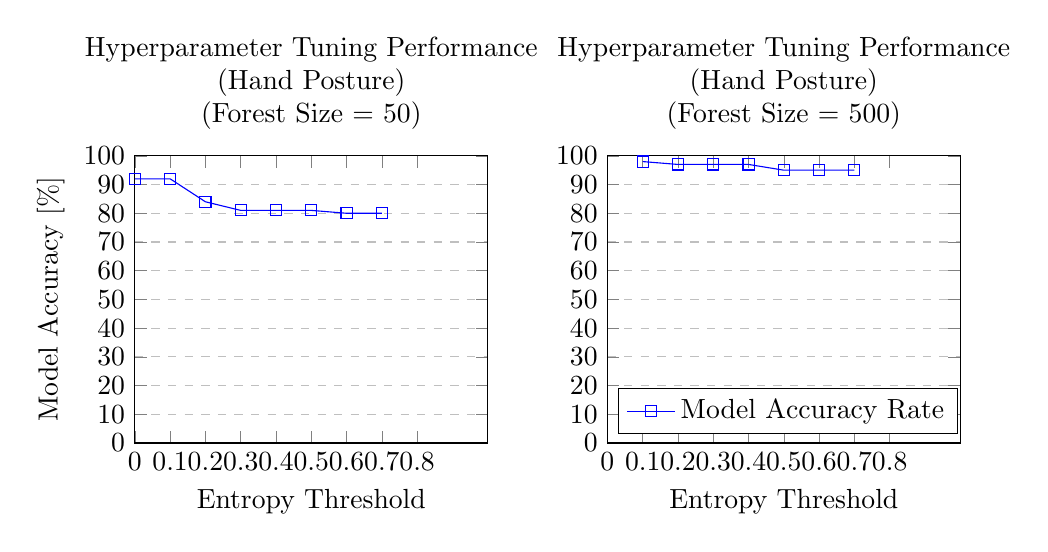
\begin{tikzpicture}[every axis/.append style={width=0.5\linewidth,title style={align=center}}]
  
  \begin{axis} [
    name = axis1,
    title = {Hyperparameter Tuning Performance \\ (Hand Posture) \\ (Forest Size = 50)},
    xlabel = {Entropy Threshold},
    ylabel = {Model Accuracy [\%]},
    xmin = 0, xmax = 1,
    ymin = 0, ymax = 100,
    xtick={0,0.1,0.2,0.3,0.4,0.5,0.6,0.7,0.8},
    ytick={0,10,20,30,40,50,60,70,80,90,100},
    legend pos = south west,
    ymajorgrids=true,
    grid style = dashed
    ]
    \addplot[
    color = blue,
    mark = square,
    ]
    coordinates {
      (0.0,92)(0.1, 92)(0.2, 84)(0.3,81)(0.4,81)(0.5,81)(0.6,80)(0.7,80)
    };
  \end{axis}
  
  \begin{axis} [
    at={(axis1.outer north east)}, anchor=outer north west,
    name=axis2,
    title = {Hyperparameter Tuning Performance \\ (Hand Posture) \\ (Forest Size = 500)},
    xlabel = {Entropy Threshold},
    %ylabel = {Model Accuracy [\%]},
    xmin = 0, xmax = 1,
    ymin = 0, ymax = 100,
    xtick={0,0.1,0.2,0.3,0.4,0.5,0.6,0.7,0.8},
    ytick={0,10,20,30,40,50,60,70,80,90,100},
    legend pos = south west,
    ymajorgrids=true,
    grid style = dashed
    ]
    \addplot[
    color = blue,
    mark = square,
    ]
    coordinates {
      (0.1,98)(0.1, 98)(0.2, 97)(0.3,97)(0.4,97)(0.5,95)(0.6,95)(0.7,95)
    };
    \legend{Model Accuracy Rate}
  \end{axis}
  
\end{tikzpicture}

\caption{Model Complexity Curves (Hand Posture Data)} \label{fig:MCCurves_Hand}
\end{figure}

\begin{figure} %
  \centering
  \subfigure[n\_estimators = 10] {%
    \label{fig:Boosting Learning Curve alpha = 0}%
    \includegraphics[height=2in]{Boosting/output/Boost_Accuracy_Rates.png}}%
  \hspace{8pt}%
  \subfigure[n\_estimators = 10]{%
    \label{fig:Boosting Learning Curve alpha = -1}%
    \includegraphics[height=2in]{Boosting/output/Boosting_Accuracy_Rates2.png}}
  \caption{Learning Curves:  Training vs. Validation Accuracy w/ Varying Training Set Size}\label{fig:Boosting Learning Curves}
\end{figure}

\begin{figure} %
  \centering
  \subfigure[alpha = -1, n\_est = 20, learning rate = 0.02] {%
    \label{fig: Boosting w/ Hyperparameters 1}%
    \includegraphics[height=1.9in]{Boosting/output/Boosting_Accuracy_Rates3.png}}%
  \hspace{8pt}%
  \caption{Learning Curves:  Training vs. Validation Sets w/ Varying Learning Rate}\label{fig:Boosting Model Complexity Curves}
\end{figure}


\section{SVM \& k-Nearest Neighbors}
We run an \textbf{SVM} model twice for each dataset- A linear SVM to start, and then an SVM with a RBF kernel for each data set. SVM, on average took considerable amount of time to train, while kNN was almost instant.  We also run a \textbf{kNN} analysis by varying our $k$ parameter, our loss function hyperparameter (Euclidean vs. Manhattan distance), and weight distance.  

\subsection{Learning Curves Analysis}

\textbf{Hand Posture Data}:
In Figure \ref{fig:Linear SVM Learning Curve}, we see that the \textbf{SVM} model performed poorly.  To start, our training data just barely reaches 50\% accuracy.  A large part of this results is due to the high dimensional nature of our data.  Our SVM is drawing the best fit line amongst all dimensions, and it is NOT able to reasonably classify the given data points.  This is further evidenced by tuning alpha, which is a regularization parameter that will aid in misclassifications (lower the value, the ``broader the street'').  However, according to \ref{fig: Linear SVM Learning Curve 2} even with an alpha of 0.0001, our results did not improve that much.  On the other hand, our \textbf{kNN} model performed very well, and was fairly quick to converge around \textbf{98\%} accuracy.  Furthermore, our model was not sensitive to our specification of $k$, and $k=1$ performed just as well as $k=10$.  This suggests our high dimensional data contains inherent ``clusters'' of classes.  The figure in Figure \ref{fig:kNN Learning Curves} shows the results with the aforementioned specifications, but letting our $k$ vary from 10 to the optimum $k=1$ outputted via $GridSearchCV.best\_params\_$.

\begin{figure} %
  \centering
  \subfigure[kNN k = 10] {%
    \label{fig:kNN Learning Curve k = 10}%
    \includegraphics[height=2in]{KNN/output/kNN_Accuracy_Rates.png}}%
  \hspace{8pt}%
  \subfigure[kNN k = 1]{%
    \label{fig:kNN Learning Curve k = 1}%
    \includegraphics[height=2in]{KNN/output/kNN_Accuracy_Rates2.png}}
  \caption{Hand Posture kNN:  Training vs. Validation Accuracy w/ Varying Training Set Size}\label{fig:kNN Learning Curves}
\end{figure}

\begin{figure} %
  
  \centering
  \subfigure[SVM: alpha = 1] {%
    \label{fig:Linear SVM Learning Curve}%
    \includegraphics[height=2in]{SVM/output/SVM_Accuracy_Rates.png}}%
  \hspace{8pt}%
  \subfigure[SVM: alpha = 0.0001]{%
    \label{fig:Linear SVM Learning Curve 2}%
    \includegraphics[height=2in]{SVM/output/SVM_Accuracy_Rates2.png}}
  \caption{Hand Posture SVM:  Training vs. Validation Accuracy w/ Varying Training Size}\label{fig:SVM Learning Curves}
\end{figure}

\textbf{Credit Approval Data}:
The \textbf{kNN and SVM} models didn't work quite well for our small Credit Approval dataset, mainly due to lack of convergence.  For one, it was hard to achieve convergence using \textbf{kNN}, suggesting overfitting.  This result is contrary to the results we saw on the larger Hand Posture dataset (Figures \ref{fig:kNN Learning Curves}). However, \textbf{SVM} on the smaller Credit Approval dataset performed better in terms of accuracy (80\%) when compared to the larger Hand Posture dataset. 

\begin{figure} %
  \centering
  \subfigure[kNN k = 10] {%
    \label{fig:CC kNN Learning Curve k = 10}%
    \includegraphics[height=2in]{KNN/output/CCApproval_Accuracy_Rates.png}}%
  \hspace{8pt}%
  \subfigure[kNN k = 1]{%
    \label{fig:CC kNN Learning Curve k = 1}%
    \includegraphics[height=2in]{KNN/output/CCApproval_Accuracy_Rates2.png}}
  \caption{Credit Approval kNN:  Training vs. Validation Accuracy w/ Varying Training Set Size}\label{fig:CC kNN Learning Curves}
\end{figure}

\begin{figure} %
  \centering
  \subfigure[SVM: alpha = 0.1] {%
    \label{fig:CC Linear SVM Learning Curve}%
    \includegraphics[height=2in]{SVM/output/CC_SVM_Accuracy_Rates.png}}%
  \hspace{8pt}%
  \subfigure[SVM: alpha = 0.0001]{%
    \label{fig:CC Linear SVM Learning Curve 2}%
    \includegraphics[height=2in]{SVM/output/CC_SVM_Accuracy_Rates2.png}}
  \caption{Credit Approval SVM:  Training vs. Validation Accuracy w/ Varying Training Size}\label{fig:SVM Learning Curves}
\end{figure}

\subsection{Model Complexity Analysis}
\textbf{Hand Posture Data}:  We can resort to using an SVM with RBF kernel, instead of a linear SVM to dissect our high dimensional data.  However, this comes at the expense of \textbf{very} large computation times.  Figure \ref{fig: SVM 1)} shows a reasonably well accuracy, with hyperparameters gamma = 10, and alpha = 0.001.  The mere presence of an RBF kernel drastically improved our model, and adjusting how much each data point contributes to the formation of a decision boundry (gamma) allows us to squeeze out more accurate classifications, as shown in Figure \ref{fig: SVM 2}.

We can add complexity by altering the distance measure (between Euclidean \& Manhattan) as well as adjusting our treatment of distance weights of training data.  By ``discounting'' training data points that are farther away from the query data point, we are effectively prioritizing the classification of the query point based on proximity, rather than prioritizing solely based on aggregate average classification of \textbf{all} training points (which is the case in the ``uniform'' distance weighting scenario).  


\begin{figure} %
  \centering
  \subfigure[Gamma = 10, alpha = 0.001] {%
    \label{fig:SVM 1}%
    \includegraphics[height=1.9in]{SVM/output/Hand_RBF_Accuracy_Rates.png}}%
  \hspace{8pt}%
  \subfigure[Gamma = 1000, alpha = 0.001]{%
    \label{fig:SVM 2}%
    \includegraphics[height=1.9in]{SVM/output/SVM_Accuracy_Rates4.png}}
  \caption{Learning Curves:  Training vs. Validation Sets w/ Varying Learning Rate}\label{fig:SVM Complexity Curves}
\end{figure}

\begin{figure} %
  \centering
  \subfigure[kNN w/ Manhattan, Weighted Distance]{%
    \label{fig:kNN Complexity Manhattan, Weighted Distance}%
    \includegraphics[height=2in]{KNN/output/kNN_Accuracy_Rates4.png}}
  \hspace{8pt}%
  \subfigure[kNN w/ Manhattan, Weighted Distance (k=5000)]{%
    \label{fig:kNN Complexity Manhattan, Weighted Distance (k=5000)}%
    \includegraphics[height=2in]{KNN/output/kNN_Accuracy_Rates5.png}}
  \caption{Complexity Curves:  Training vs. Validation Accuracy w/ Varying k }\label{fig:kNN Complexity Curves}
\end{figure}

Using the figure \ref{fig:kNN Learning Curve k = 10} as a reference (which uses Uniform Distancing), you can see a subtle, yet important change in the accuracy of our validation set when using \textbf{Weighted Distance} as a hyper-parameter.  Namely, figure \ref{fig:kNN Complexity Manhattan, Weighted Distance} shows decreased performance for almost every training set sample size, reaching a maximum validation accuracy rate of 88\%.  Uniform distancing provides slightly better performance, as opposed to discounting data points further away from a test point's nearest neighbor.  Logically, this makes sense- a single instance of a hand gesture is subject to measurement bias.  By discounting all the other finger marker measurements, which also was subjected to measurement bias, we are not letting the model take this type of error into account.  Instead, the distance weighted model is simply placing a higher emphasis on the closest points to make an assessment of hand posture- a misplaced emphasis which most likely took outlier data points from other hand gesture readings, and misclassified our query point as such.  Lastly, it is worth noting that no combination of parameter + hyper-parameter tuning was able to correct the overfitting issue.  My initial hypothesis was to blow up k to 5000 as shown in \ref{fig:kNN Complexity Manhattan, Weighted Distance (k=5000)}, but it didn't do much- it just nearly blew up my laptop.  In fact, it ended up doing worse.

\textbf{Credit Approval Data}:  Looking at figure \ref{fig:CC SVM Complexity Curves}, we can clearly see the overfitting when setting Gamma to 0.1 \& Alpha to 0.001.  The overfitting was ``fixed'' when we set the Gamma to 100.  In essence, the margins set forth by the L2 Loss function need to be wide for our Credit Approval data to overcome overfitting.  While we couldn't overcome overfitting in the much larger dataset, allowing the margins to be flexible in our smaller Credit Approval dataset seems to be the wise choice.  

\begin{figure} %
  \centering
  \subfigure[Gamma = 0.1, alpha = 0.001] {%
    \label{fig:CC_RBF_Accuracy_Rates}%
    \includegraphics[height=1.9in]{SVM/output/CC_RBF_Accuracy_Rates.png}}%
  \hspace{8pt}%
  \subfigure[Gamma = 100, alpha = 0.001]{%
    \label{fig:SVM 2}%
    \includegraphics[height=1.9in]{SVM/output/CC_RBF_Accuracy_Rates2.png}}
  \caption{Learning Curves:  Training vs. Validation Sets w/ Varying Learning Rate}\label{fig:CC SVM Complexity Curves}
\end{figure}

\section{Artificial Neural Networks}

\subsection{Learning Curves Analysis}
\textbf{Credit Approval Data}  We can tune our parameters by increasing both the depth, and size of our hidden layers.  Looking at figure \ref{fig:ANN Complexity Curves}, you can see that our ANN model with 3 hidden layers, each of size 30 performs slightly better at lower iterations, but worse at higher number of iterations, as compared to specifying 1 hidden layer of size 1 node.  The overall conclusion here is that the simple model with 1 hidden layer using 1 node actually performs better than one with more hidden layers at high number of iterations.

The first figure in \ref{fig:ANN Complexity Curves} produces very promising results.  With 30 nodes in each of the 3 Hidden Layers, we can only achieve 80\% fit in the training set, and 80\% in the test set no matter the number of weight-adjustment iterations (backpropogation).  The performance is quite poor all around.  The right graph uses the $basicResults.best\_params\_$ method made available in scikitlearn to choose the best parameter for our ANN.  The best parameters are:  (1) L2 Penalty: 0.00316 (2) Hidden Layer Depth: 1 (3) Hidden Layer Size: 1 (4) Activation Function: RELU.  Note that the figure on the right suggests we can reach a generalizable and accurate (88\% test accuracy rate with 90\% training accuracy rate) model with anywhere between 1,024 to 2048 weight-adjustment iterations.  Figure \ref{fig:ANN Complexity Curve} also highlights the importance of back-propogation.  Giving our model time to make iterative adjustments to the weights drastically improves the model.

\begin{figure} %
  \centering
  \subfigure[\centering ANN: Credit Card Data \\
  \centering 3 Hidden Layers, 30 Nodes Each] {%
    \label{fig:ANN Complexity Curve Layer30x3}%
    \includegraphics[height=1.9in]{Neural_Nets/output/ANN_Accuracy_Rates3.png}}%
  \hspace{8pt}%
  \subfigure[[\centering ANN: Credit Card Data \\
  \centering 1 Hidden Layer, 1 Nodes]{%
    \label{fig:ANN Complexity Curve}%
    \includegraphics[height=1.9in]{Neural_Nets/output/ANN_Accuracy_Rates4.png}}
  \caption{ANN Credit Approval Complexity Curves:  Testing vs. Validation Sets w/ Varying Depth and Number of Hidden Layer Nodes}\label{fig:ANN Complexity Curves}
\end{figure}  

\subsection{Model Complexity Analysis}
\textbf{Credit Approval Data}  To get a basic understanding of how our model performed, we first start off with a ``basic'' neural net with the following specifications:  (1) 1 Hidden Layer of size 30.  (2) Activation Function = 'relu' (rectified linear unit function, returns f(x) = max(0,x)) (3) L2 Regularization Alpha = 0.  The figure in Figure \ref{fig:ANN Learning Curves} shows the results with the aforementioned specifications, but letting our L2 Regularization/Penalty term to vary between 0 \& 10.
Recall that the L2 Norm is essentially a squared error specification, and by it's nature, penalizes weights in a manner to reduce the likelihood of fitting the noise of the training data.

\textbf{Hand Posture Data}  My preconceived notion was that a larger dataset would fare better using ANN, since more features and more instances should allow for better opportunities to classify.  But this turned out not to be the case.  With many different combinations of tuning, the best validation score  I was able to achieve was 78\% as shown in Figure \ref{fig:Posture Complexity Curve}.  I didn't get reasonable results until I switched the Learning Rate hyperparameter from 'Constant' to 'Adaptive,' which suggests a finer tuning of alpha was necessary.  Given this result, I changed alpha to 0.0001, but counterintuitively, that caused my results to again suffer.  Eventually, I arrived at a 0.1 alpha specification (with adaptive learning rates) to achieve 78\%.

\begin{figure} %
  \centering
  \subfigure[L2 Regularization = 0] {%
    \label{fig:ANN Learning Curve L2 = 0}%
    \includegraphics[height=1.9in]{Neural_Nets/output/ANN_Accuracy_Rates.png}}%
  \hspace{8pt}%
  \subfigure[L2 Regularization = 10]{%
    \label{fig:ANN Learning Curve L2 = 10}%
    \includegraphics[height=1.9in]{Neural_Nets/output/ANN_Accuracy_Rates2.png}}
  \caption{Learning Curves:  Training vs. Validation Sets w/ Varying Alpha (L2-Norm)}\label{fig:ANN Learning Curves}
\end{figure}


\begin{figure} %
  \centering
  \subfigure[\centering ANN: Hand Posture Data \\
  \centering 1 Hidden Layer, 50 Nodes, Adaptive LR, 0.1 Alpha] {%
    \label{fig:Posture Complexity Curve}%
    \includegraphics[height=1.9in]{Neural_Nets/output/Posture_Accuracy_Rates.png}}%
  \hspace{8pt}%
  \subfigure[[\centering ANN: Hand Posture Data \\
  \centering 1 Hidden Layer, 50 Nodes, Constant LR, 0.1 Alpha]{%
    \label{fig:Posture Complexity Curve2}%
    \includegraphics[height=1.9in]{Neural_Nets/output/Posture_Accuracy_Rates2.png}}
  \caption{ANN Hand Posture Complexity Curves:  Testing vs. Validation Sets w/ Constant + Adaptive Learning Rate Behavior}\label{fig:ANN Complexity Curves}
\end{figure}

\end{document}